\Titular%
{O misterio da materia escura}%
{Pablo Falgueras Casarejos}%
{divulgacion}%
{O descubrimento da maior parte da materia do universo e o enigma da súa composición.}%


\begin{refsection}


\begin{multicols}{2}


Dende os anos trinta do século XX sabemos que no universo hai algún tipo de materia invisible aos nosos instrumentos debido aos efectos que esta ten no seu entorno. Un dos primeiros en obter probas firmes sobre este feito foi o físico Fritz Zwicky no ano 1933 mentres estudada o Cúmulo de Coma, un cúmulo formado por unhas mil galaxias na constelación de Coma Berenices, a algo máis de 300 millóns de anos luz. Zwicky mediu as velocidades das galaxias do cúmulo e atopou que eran moito maiores do esperado só tendo en conta a materia visible, de feito, chegaban a superar a velocidade de escape estimada para o cúmulo. En consecuencia, propuxo que debía existir algún tipo de “materia escura” que non podiamos observar responsable do movemento anómalo das galaxias. Non obstante, este achado caeu no esquecemento ata catro décadas despois. Hoxe en día sábese que Zwicky sobreestimou a cantidade de materia escura porque non tivo en conta o gas intergaláctico (aínda non descuberto), o cal aporta a maior parte da masa do cúmulo. 

Xa na década dos 70, a astrónoma Vera Rubin xunto con Kent Ford, analizando a velocidade de rotación de estrelas individuais en galaxias espirais, atoparon o mesmo resultado que Zwicky nas galaxias do Cúmulo de Coma corenta anos antes. A velocidade das estrelas era demasiado alta: en vez de diminuír coa distancia, mantíñase aproximadamente constante. De novo, Rubin pensou que existía máis materia da visible, a cal se acumulaba na rexión exterior (halo) das galaxias. As estimacións da cantidade de materia escura suxerían que podía ser ata dez veces máis abundante que a materia ordinaria (ou bariónica, formada por barións).

Ao longo dos anos, presentáronse novas probas que apuntan á existencia desta materia escura. Por exemplo, estudando a velocidade do gas das galaxias, e non a velocidade das súas estrelas, pódese apreciar unha maior anomalía nela. Isto débese a que o gas exténdese máis aló na periferia da galaxia que as estrelas, aínda que tardou en ser descuberto porque emite principalmente en raios X debido á súa alta temperatura. Outros obxectos do halo galáctico cuxa velocidade presenta a mesma irregularidade son os cúmulos globulares, cúmulos moi antigos formados por decenas ou centos de miles de estrelas.

Por outra banda, dende a publicación da teoría da relatividade xeral de Einstein sábese que unha masa deforma o espazo-tempo, polo que pode curvar a traxectoria da luz producindo un fenómeno coñecido como lente gravitacional. Esto prodúcese cando un obxecto masivo (unha galaxia ou cúmulo de galaxias, por exemplo) interponse entre unha fonte de luz (outra galaxia distante) e o observador. Se é o caso, pódese observar a galaxia distante distorsionada debido ao efecto de lente gravitacional do corpo interposto. Estudando como ese corpo curva a traxectoria da luz pódese estimar a cantidade e distribución de masa que produce a lente gravitacional. Grazas a isto, obsérvase que unicamente a materia bariónica non podería producir as lentes gravitacionais estudadas, senón que é necesaria a presencia de máis masa para conseguilo.\\

\begin{center}
    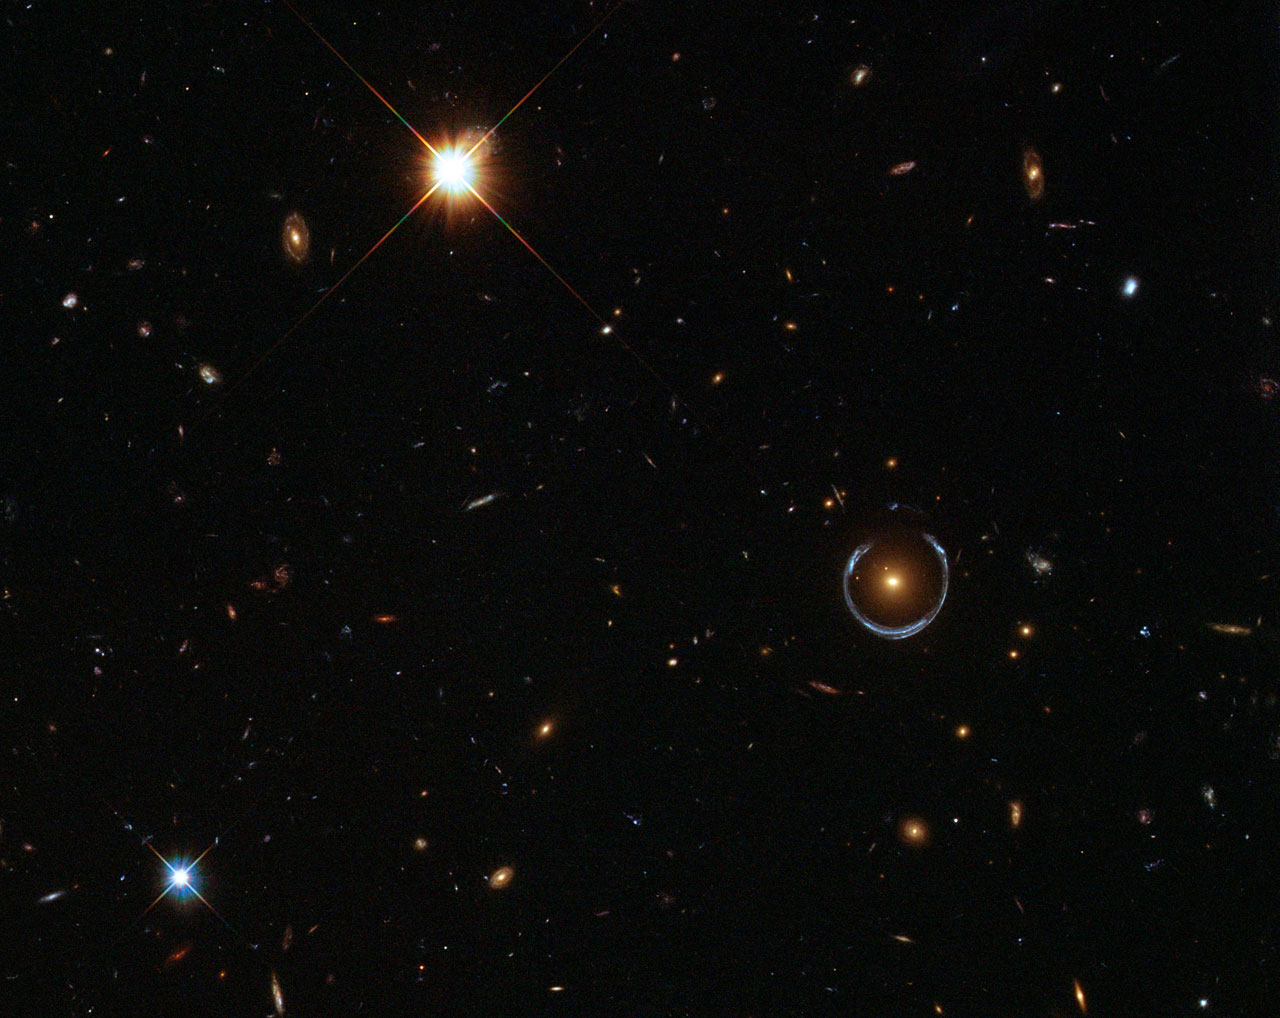
\includegraphics[width=0.9\linewidth]{revistas/002/imaxes/materiaescura1.png}
    \captionof{figure}{LRG 3-757 ou a “ferradura cósmica”, un exemplo das lentes gravitacionais coñecidas como aneis de Einstein.\cite{hubbleNASA}}
\end{center}


Outra proba provén da radiación do fondo cósmico de microondas (Cosmic Microwave Background, CMB, en inglés), radiación emitida durante a chamada “recombinación” uns 380 000 anos despois do Big Bang. Analizando as fluctuacións de temperatura do CMB estímase que a dendisade de materia (escura e ordinaria) do universo atópase en torno ao 32\% da súa densidade crítica, o cal está en perfecto acordo coas observacións, das que se obtén que a materia bariónica supón un 5\% da densidade crítica e a materia escura un 27\%. Por certo, pénsase que a contribución da “enerxía escura” (non materia!) é igual ao 68\% restante, polo que a densidade do universo sería igual á súa densidade crítica e a xeometría deste sería plana.

Sobre as súas características, sábese que a materia escura debe de ser “fría”, é dicir, que a velocidade das súas partículas é moito menor que a velocidade da luz. Se non fose así, o colapso gravitatorio da materia no universo temperán tería sido menos eficiente e non existiría a estrutura a gran escala actual. Tamén debe ser estable, porque a cantidade de materia escura actual debe de ser aproximadamente a mesma que a do universo temperán. Ademais, a materia escura non interacciona coa materia bariónica nin consigo mesma (a excepción da gravidade) ou o fai de forma moi débil. Un claro exemplo preséntase noutro cúmulo de galaxias, o denominado Cúmulo Bala. En realidade, trátanse de dous cúmulos en colisión, os cales xa se atravesaron hai millóns de anos. A partir de observacións en raios X, apréciase que o gas intergaláctico (en vermello na Figura 2) está rezagado respecto aos cúmulos, o cal prodúcese pola fricción das nubes de gas  ao chocar. O interesante é que debido aos efectos de lente gravitacional pódese saber a distribución de materia escura (en azul), que si está superposta ao cúmulo (non rezagada). Isto quere dicir que cando os cúmulos colisionaron, a materia escura atravesou as nubes de gas e a si mesma sen apenas interaccionar, doutro xeito tamén se retrasaría como o gas. \\

\begin{center}
    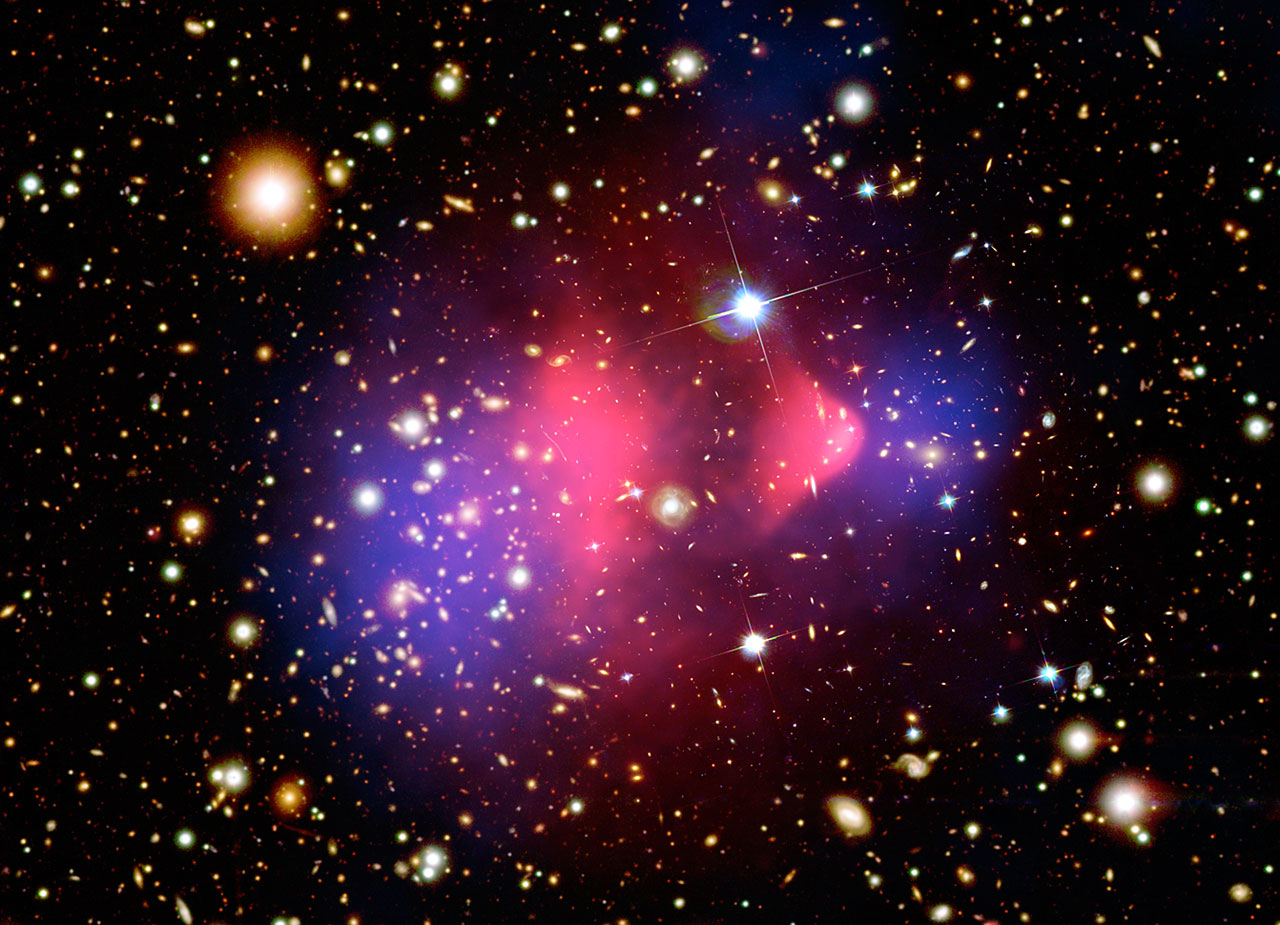
\includegraphics[width=0.85\linewidth]{revistas/002/imaxes/materiaescura2.png}
    \captionof{figure}{O Cúmulo Bala na constelación de Carina. En vermello, a emisión en raios X do gas intergaláctico; en azul, a distribución de materia escura obtida a través dos efectos de lente gravitacional.\cite{hubbleNASA2}}
\end{center}

Iso si, se ben parece estar bastante claro que a materia escura existe aínda que non a vexamos, no que respecta á súa composición a situación é moi distinta. A día de hoxe non se coñece con certeza de que está feita, mais hai moitos candidatos a materia escura. En primeiro lugar, poderíamos preguntarnos se se trata de materia ordinaria que por algunha razón resulta invisible, o cal xa está prácticamente descartado. Por exemplo, quizais sería algún obxecto compacto coma un MACHO (Massive Astrophysical Compact Halo Object), isto é, buracos negros, planetas errantes, asteroides, etc., mais os seus efectos gravitacionais serían diferentes aos da materia escura (o caso dos buracos negros primordiais aínda se está a estudar). Tampouco poden ser nubes de gas escuras (como as nebulosas escuras), pois absorberían a luz de estrelas ou galaxias distantes, o cal non observamos; a materia escura é transparente á luz. Os neutrinos descartámolos igualmente porque debido á súa ínfima masa terían velocidades moi altas e serían “quentes”, non fríos.

Algúns dos candidatos máis prometedores son os WIMPs (Weakly Interacting Massive Particle, ou partículas masivas que interactúan debilmente), dos cales o neutralino é un bo exemplo. Os neutralinos son as partículas supersimétricas máis lixeiras e posúen características interesantes compatibles coas da materia escura. Outras partículas moi estudadas son os axións, que aparecen en propostas para resolver o problema CP forte na cromodinámica cuántica. Iso si, debemos recordar que neutralinos ou axións son aínda partículas hipotéticas non detectadas experimentalmente. En realidade, para responder que é a materia escura atopamos dende partículas exóticas cuxa existencia non ten demasiado apoio teórico ou a posibilidade de que haxa dimensións extras, ata a simple ausencia de materia escura. Estas últimas teorías (chamadas MOND) suxiren unha modificación no comportamento da gravidade a grandes distancias, o cal explicaría as altas velocidades das estrelas ou galaxias xa comentadas. Non obstante, estas teorías non poderían explicar os efectos de lente gravitacional observados.

En definitiva, temos moitas probas da existencia da materia escura e coñecemos algunhas das súas características, mais o seu constituínte é incerto. Aínda que xa están descartados algúns candidatos e moitos outros probablemente descartaranse no futuro, terase que seguir investigando para resolver este enigma


\nocite{alberto2021materiaescura}
\nocite{krauss5esencia}
\nocite{hubbleNASA}
\nocite{hubbleNASA2}
\printbibliography


\end{multicols}
\end{refsection}